% DEFINICIONES (ANTECEDENTES)
% def pasos y corridas
% controlador
% vemos en particular problemas non-blocking (i.e. loop para ganadores, no-controlables no joden)
% estados ganadores y perdedores (estados desde donde hay una estrategia==controlador ganadora/perdedora)
%-------------------------------------------------------
\begin{frame}{Problema de control non-blocking}
    \begin{block}{¿Cuál es la entrada de un problema de control?}
        \begin{itemize}
          \item conjunto de autómatas (la composición de ellos es la planta completa que no queremos calcular)
          \item acciones controlables y no controlables
          \item estados marcados u objetivos (se quiere tener la \textit{posibilidad} de visitar infinitas veces \textit{al menos uno})
        \end{itemize}
    \end{block}

    \begin{block}{¿Qué devuelve?}
        Una estrategia ganadora (llamada controlador) o afirmación de que no existe.
    \end{block}

\end{frame}
%-------------------------------------------------------
\begin{frame}{Acciones, pasos y corridas (run)}
    \begin{figure}
        \begin{overprint}
        \onslide<1>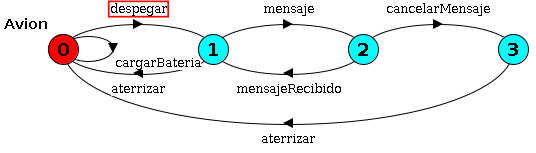
\includegraphics[width=\textwidth]{figures/1accion.png} 
        \onslide<2>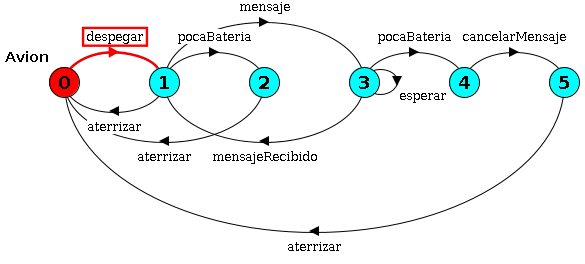
\includegraphics[width=\textwidth]{figures/2paso.png} 
        \onslide<3->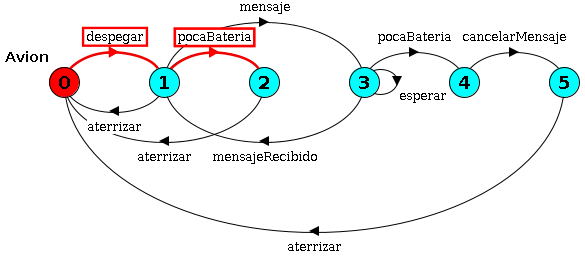
\includegraphics[width=\textwidth]{figures/3run.png} 
        \end{overprint}
    \end{figure}

    \begin{itemize}
     \item Acción es una transición entre los estados.
     \pause
     \item Un paso es $t \step{\l}{T} t'$, toma en cuenta el estado de partida y llegada.
     \pause
     \item Una corrida de una palabra $w = \l_0,\ldots,\l_k$ en $T$, es $t_0 \runw{w}{T} t_{k+1}$, es decir, varios pasos.
    \end{itemize}
    
\end{frame}
%-------------------------------------------------------
\begin{frame}{Controlador}
    \begin{figure}
     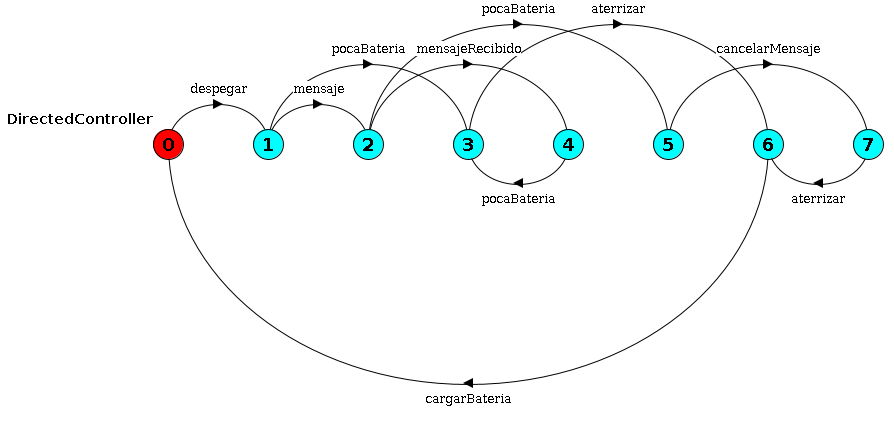
\includegraphics[width=\textwidth]{figures/director.png}
    \end{figure}

    Es una restricción de la planta (la composición de todos los autómatas) que cumple las reglas:

    \begin{itemize}
     \item Puede prohibir pasos controlables.
     \item Debe mantener todos los no-controlables.
     \item Todas las corridas posibles en la planta restringida pasan por algún estado marcado.
    \end{itemize}
\end{frame}
%-------------------------------------------------------
\begin{frame}{Estados ganadores y perdedores}
    Si existe un controlador comenzando desde un estado, es decir, existe estrategia ganadora a partir del estado, entonces lo consideramos estado ganador. 
    Caso contrario, el estado es perdedor y debemos evitarlo.
    
    [Agregar ejemplos imágenes]
    
    \begin{block}{Observación}
        En particular nos interesa mucho si el estado inicial es ganador/perdedor, ya que eso nos dice si existe o no un controlador \textit{empezando} desde ahí.
    \end{block}

\end{frame}
%-------------------------------------------------------
\begin{frame}{Particularidades de non-blocking}
    \begin{block}{Necesitamos un ciclo (loop) para ganar}
        a qué nos referimos con loop\\
        La única forma de visitar infinitas veces un estado es que la corrida sea un ciclo.
    \end{block}
    
    [pictures pictures and more pictures]
\end{frame}
%-------------------------------------------------------
